\newpage
\section{Three-dimensional normal injector}
\label{chapter-3Dinjector}
%
This test case investigates the flow structure of an air jet injected into an air cross-flow over a flat plate. The case is based on the experimental and computational validation performed by Viti et. al.~\cite{schetz2009} regarding a RANS solver utilising the $k$-$\omega$ turbulence model. 

Viti~\cite{schetz2009} utilises the experimental pressure results produced by Wallis~\cite{wallis2001} in an effort to validate the simulation, however noted that due to the large experimental errors associated with the Pressure-Sensitive Paint (PSP) used, an exhaustive quantitative analysis would not be possible. Instead, a limited qualitative validation using Schlieren imagery by Viti et. al.~\cite{viti2004} would be conducted as a result.

%------------------------------------------------------------------
\subsection{Details of flow problem}
%\label{}
Figure~\ref{f:tc3:scheme} indicates the basic schematic for Test Case 3. The flow regime features a flat plate with a $4.76$\,mm diameter circular injector, injecting Mach 1 air into a Mach 4 air cross-flow. 
%
\begin{figure}[htbp]
 \begin{center}
  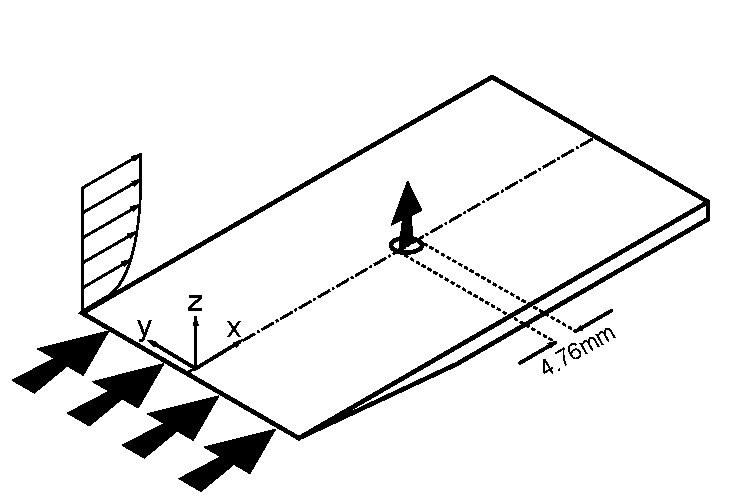
\includegraphics[width=9cm]{./chap8-3Dinjector/figs/inject-schematic.pdf}
  \caption{Basic Schematic for Injector Simulation.}
  \label{f:tc3:scheme}
 \end{center}
\end{figure}
%
The flat plate upstream of the injector has a length of $76.2$\,mm, and features a $16.5$\,mm thick incoming boundary layer. The upstream length allows the cross-flow boundary layer to further develop before interacting with the injector flow. The cross-flow-injector interaction will result in the formation of the characteristic shocks (interference, Lambda, bow, barrel and reflected) and Mach disk, common to this flow regime.

Inflow and initial flow conditions were set using values specified by Viti~\cite{schetz2009}, and are listed in Table~\ref{t:tc3:initial}. Conditions for the injector flow were also specified, and are listed in Table~\ref{t:tc3:jet}. Pressure, temperature and Mach number were supplied, and velocity was calculated using Mach number relations, by calculating sound speed using the flow temperature (Equation~\ref{e:machnumrel}). Density was determined using the ideal gas law (Equation~\ref{e:idealgaslaw}).
\begin{equation}
  \label{e:machnumrel}
  U_\infty = M_\infty \times \sqrt{\gamma \times R \times T_\infty}
\end{equation}
\begin{equation}
  \label{e:idealgaslaw}
  \rho_\infty = \frac{P_\infty}{R \times T_\infty}
\end{equation}
%
\begin{table}[htbp]

  \caption{3D Injector Initial \& Inflow (Freestream) Conditions.}
  \label{t:tc3:initial}
    \begin{center}
    \begin{tabular}{cccl}
  \hline\hline
     Property  & Value & Units \\
  \hline
    $P_\infty$  & $7.1\times10^3$ & Pa  \\
    $U_\infty$  & $671.92$ & m/s  \\
    $T_\infty$  & $70.3$ & K  \\
    $\rho_\infty$  & $0.352$ & kg/m$^3$  \\
  \hline\hline
  \end{tabular}
  \end{center}
\end{table}
%
%
\begin{table}[htbp]
  \caption{3D Injector Jet Conditions.}
  \label{t:tc3:jet}
  \begin{center}
  \begin{tabular}{cccl}
  \hline\hline
     Property  & Value & Units \\
  \hline
    $P_J$  & $2.006\times10^6$ & Pa  \\
    $U_J$  & $323.67$ & m/s  \\
    $T_J$  & $261$ & K \\
    $\rho_J$  & $26.77$ & kg/m$^3$  \\
  \hline\hline
  \end{tabular}
  \end{center}
\end{table}

Viti~\cite{schetz2009} assumed an initial turbulence intensity of $5\%$ and that the turbulent viscosity was $10\%$ of the laminar viscosity ($\frac{\mu_{lam}}{\mu_{turb}}=10$). This allowed initial $k$ and $\omega$ values to be calculated for use in the simulation, as indicated in Table~\ref{t:tc3:turb}.
%
\begin{table}[htbp]
  \caption{3D Injector Initial (Freestream) Turbulence Properties.}
  \label{t:tc3:turb}
  \begin{center}
  \begin{tabular}{cccl}
  \hline\hline
     Property  & Value & Units \\
  \hline
    Turbulence Kinetic Energy ($k$)  & $1693.04$ & m$^2$/s$^2$  \\
    Specific Dissipation Rate ($\omega$)  & $12.54\times10^6$ & /s  \\
  \hline\hline
  \end{tabular}
  \end{center}
\end{table}
%
\subsection{Details of computational approach}
%\label{}
Viti~\cite{schetz2009} noted that an incoming boundary layer of $16.5$\,mm thickness was required for the numerical simulations. In order to achieve this, a two-dimensional `run-up' geometry was developed which was representative of a 2D $x$-$z$ slice of the fluid domain above the flat plate. 

The `run-up' was a $1.6$\,m$\times0.1524$\,m rectangular mesh, as indicated in Figure~\ref{f:tc3:runupmesh}, divided into a high resolution ($512\times152$ cells) mesh. The south face was represented by an adiabatic wall ($AdiabaticBC$), with cells clustered towards it to ensure a $y^+<1$. The north and east edges were set to open boundaries, using  $ExtrapolateOutBC$, so as to allow the oblique shock caused by the leading edge interaction to leave the domain. By interpolating a profile from the end of the 2D `run-up' at the desired 3D resolution using the developed interpolator code, the required boundary layer thickness was achieved and set as inflow for the three-dimensional simulation.
%
\begin{figure}[htbp]
 \begin{center}
  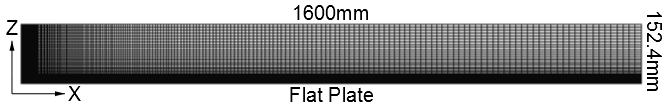
\includegraphics[width=14cm]{./chap8-3Dinjector/figs/inject-runup-mesh.png}
  \caption{3D Injector `Run-up' Mesh.}
  \label{f:tc3:runupmesh}
 \end{center}
\end{figure}
%

The second geometry comprised a $0.2769$\,m$\times0.1143$\,m$\times0.1524$\,m block with a $4.12$\,mm diameter circular injector positioned $76.2$\,mm from the leading edge (Figure~\ref{f:tc3:coordinates}), as specified by Viti~\cite{schetz2009}. The reduction in injector diameter corresponded to the implementation of a nozzle discharge coefficient ($Cd_J$), estimated by Viti~\cite{viti2002} to be $0.78$ for numerical simulations. This enabled the jet to be modelled as a step profile, with no `run-up' or inflow boundary layer.
%
\begin{figure}[htbp]
 \begin{center}
  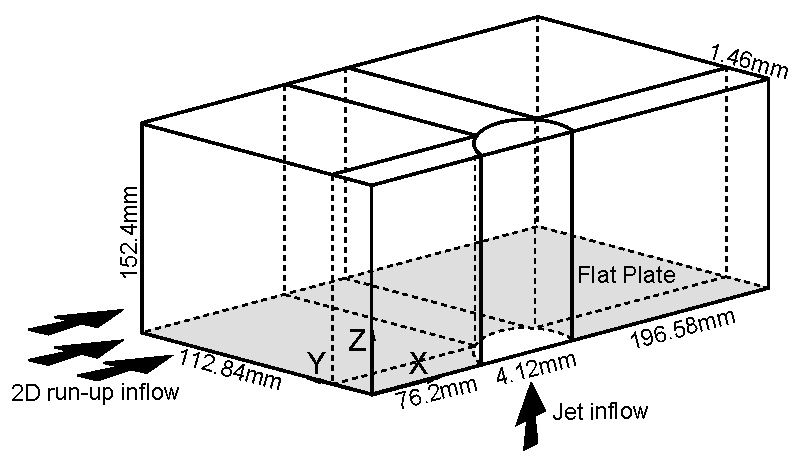
\includegraphics[width=14cm]{./chap8-3Dinjector/figs/inject-blocks.pdf}
  \caption{3D Injector Mesh Geometry (not to scale).}
  \label{f:tc3:coordinates}
 \end{center}
\end{figure}
%

The south boundary of the domain was set as a symmetry plane using the $SlipWallBC$ boundary condition, requiring only half of the injector to be modelled and simulated. The western boundaries were set to accept ghost-cell data from the 2D `run-up' simulation using the $StaticProfBC$ boundary condition. The bottom surfaces (apart from the jet) were set to adiabatic walls ($AdiabaticBC$) to allow viscous flow effects to occur, and continue the development of the incoming turbulent boundary layer. The bottom surface for the jet block was set to allow supersonic inflow perpendicular to the cross-flow using the $SupInBC$ boundary condition. All other surfaces were set as open boundaries through the use of $ExtrapolateOutBC$. 

The 3D geometry was split into a $80\times75\times80$ cell mesh ($25+5+50$ in $X$, $5+70$ in $Y$, $80$ in $Z$, $480000$ cells total, Figure~\ref{f:tc3:mesh}), with the interpolated 2D inflow profile featuring an identical vertical cell-count to ensure compatibility. Strong clustering towards the flat plate (bottom boundary) was utilised to achieve $y^+<1$. Weaker clustering was used to smooth the transitions between the half-cylinder injector block and the surrounding blocks.
%
\begin{figure}[htbp]
 \begin{center}
  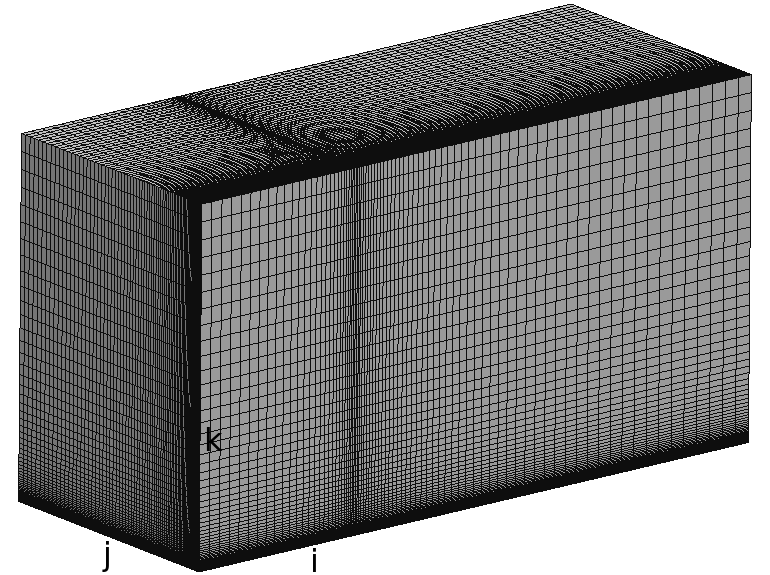
\includegraphics[width=12cm]{./chap8-3Dinjector/figs/inject-mesh.png}
  \caption{3D Injector Simulation Mesh.}
  \label{f:tc3:mesh}
 \end{center}
\end{figure}
%

The `run-up' domain was split into 16 blocks ($4\times4$) for multi-threaded Eilmer3 simulation. The 3D injector domain was split into 96 blocks ($3\times4\times8$), by breaking the main mesh into eight vertical ($k$) slices, and the larger blocks twice in the $i$ and $j$ directions. The cell-count and clustering in the $Z$ direction was identical, to ensure the 2D outflow profile correctly correlated with the 3D geometry. Block distribution was not required to be the same, as the outflow profile was extracted along a slice and then split as required.

\subsection{Results \& discussion}
%\label{}
%
\subsubsection{2D Injector `Run-up' Results}
%\label{}
%
The two-dimensional `run-up' was tested for $5$ milliseconds, approximately three flow lengths, in order to ensure the initial inflow had left the fluid domain. This required a `Barrine' simulation lasting $51$ hours ($816$ CPU-hours). 

Figure~\ref{f:tc3:runupmach} indicates pressure over the flow domain. As distance from the leading edge ($X$) increases, the boundary layer is observed to increase in thickness, as expected. An oblique shock, caused by the interaction with the flat plate leading edge, is seen leaving the flow domain at approximately $\frac{1}{3}rd$ of the plate's total length.
%
\begin{figure}[htbp]
 \begin{center}
  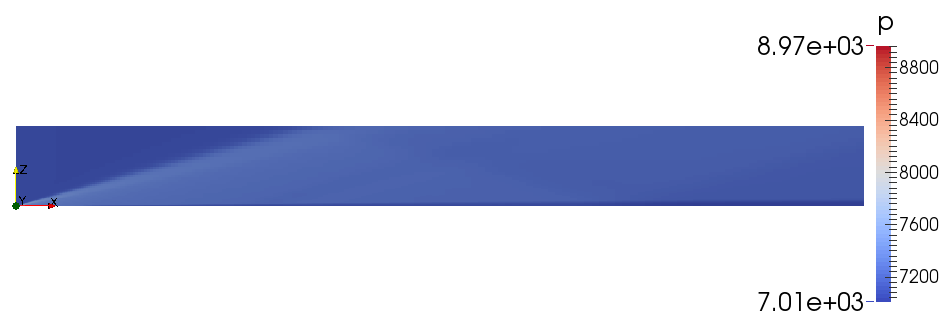
\includegraphics[width=14cm]{./chap8-3Dinjector/figs/inject-runup-pressure.png}
  \caption{2D Injector `Run-up' Pressure Data.}
  \label{f:tc3:runupmach}
 \end{center}
\end{figure}
%

The flow data at $x=1.6$\,m was interpolated to the lower 3D resolution and extrapolated into the third dimension, for use as inflow for the three-dimensional injector simulation. The boundary layer thickness indicated by the velocity profile (Figure~\ref{f:tc3:interpolatedprofile}) is $16$-$17$\,mm thick, replicating the $16.5$\,mm profile utilised by Viti~\cite{schetz2009} and ensuring adequate inflow conditions for the injector cross-flow.
%
\begin{figure}[htbp]
 \begin{center}
  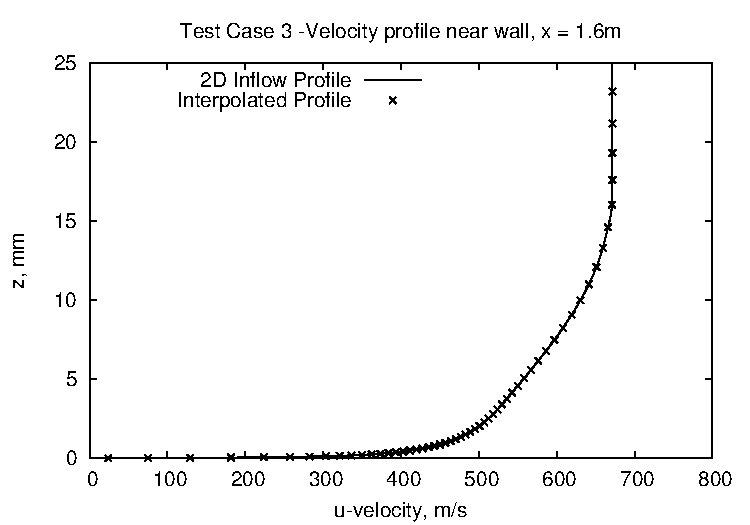
\includegraphics[width=14cm]{./chap8-3Dinjector/figs/inject-runup-vel-profile.pdf}
  \caption{2D Injector `Run-up' Interpolated Inflow Profile.}
  \label{f:tc3:interpolatedprofile}
 \end{center}
\end{figure}
%

\newpage
\subsubsection{3D Injector Results}
%\label{}
%
The three-dimensional geometry had solutions extracted at 0.758 milliseconds, after simulation on `Barrine' for 546 hours, or 3-4 weeks (the equivalent of 52416 CPU-hours).

Figure~\ref{f:tc3:injectormach} indicates Mach number over the fluid domain. As predicted, these interactions between the cross-flow and perpendicular injector flow result in the formation of a series of characteristic shocks, common to the flow scheme. 

%
\begin{figure}[htbp]
 \begin{center}
  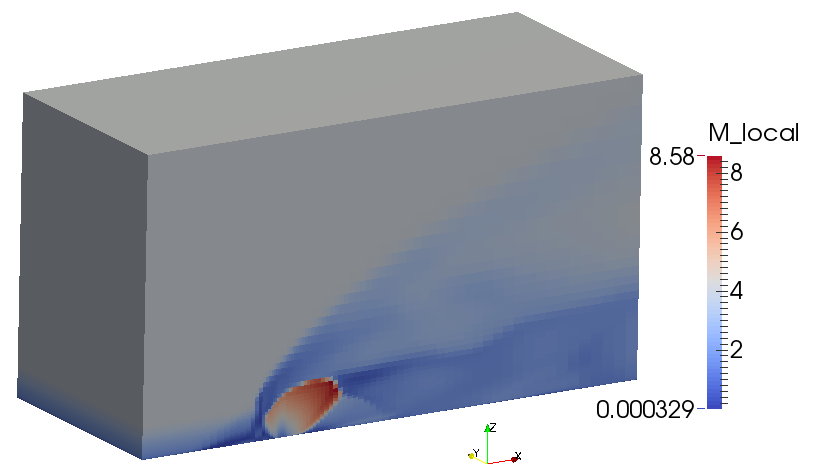
\includegraphics[width=14cm]{./chap8-3Dinjector/figs/inject-mach.png}
  \caption{3D Injector Mach Number Data.}
  \label{f:tc3:injectormach}
 \end{center}
\end{figure}
%

The sonic air injection into the Mach 4 cross-flow results in the formation of a barrel shock (high Mach number oval-shaped region), which sharply terminates in a Mach disk (edged end of oval). This is due to the jet pressure being much larger than that of the cross-flow - the jet is under-expanded. A reflected shock originates from the base of the Mach disk and barrel shock (a `triple point'), and arcs downwards to the surface of the flat plate. A bow shock forms ahead of the injector, as the barrel shock acts as a blunt body obstruction, resulting in the deflection of the supersonic cross-flow. The presence of this bow shock causes separation of the turbulent boundary layer from the surface of the flat plate, upstream of the injector.

These phenomena are more observable when compared to the computational solutions and Schlieren images obtained by Viti~\cite{schetz2009}~\cite{viti2004}, indicated in Figure~\ref{f:tc3:schetzcompare1} and~\ref{f:tc3:schetzcompare2}. Overall, the correspondence of the shock placement and size is excellent given the test time, however it is obvious that the selected resolution for the 3D injector is not sufficiently detailed. This is particularly obvious in Figure~\ref{f:tc3:schetzcompare2}, where the Mach number transitions between shocks indicate heavy aliasing/stair-casing. 

\begin{figure} [htbp]
	\centering
	\subfigure[][Viti Simulation (see Viti et. al.~\protect\cite{schetz2009}).]{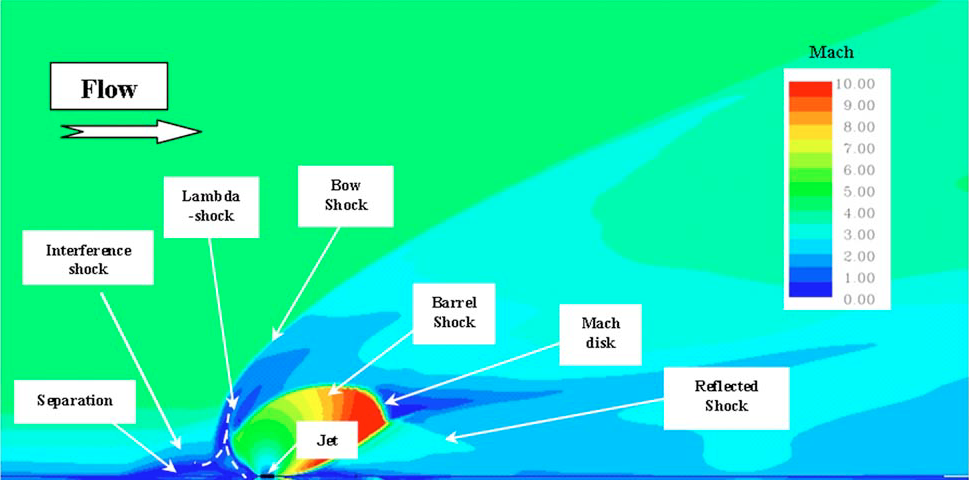
\includegraphics[width=13cm]{./chap8-3Dinjector/figs/viti-mach.png}}%
	\qquad	
	\subfigure[][Eilmer3 Simulation.]{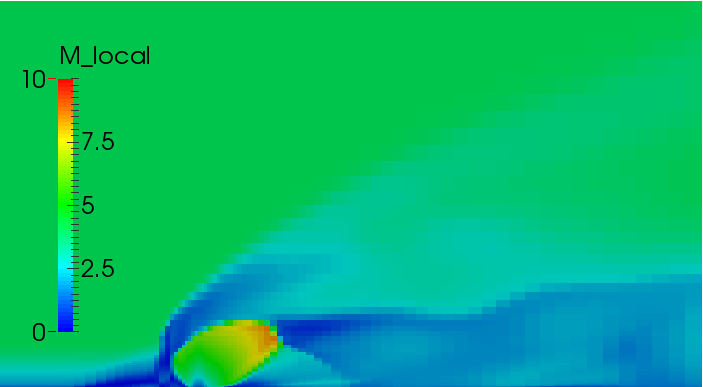
\includegraphics[width=13cm]{./chap8-3Dinjector/figs/inject-mach-profile.png}}%
	\caption{3D Injector Mach Number Comparison.}%
	\label{f:tc3:schetzcompare1}%
\end{figure}


\begin{figure} [htbp]
	\centering
	\subfigure[][Viti Simulation (see Viti et. al.~\protect\cite{schetz2009}).]{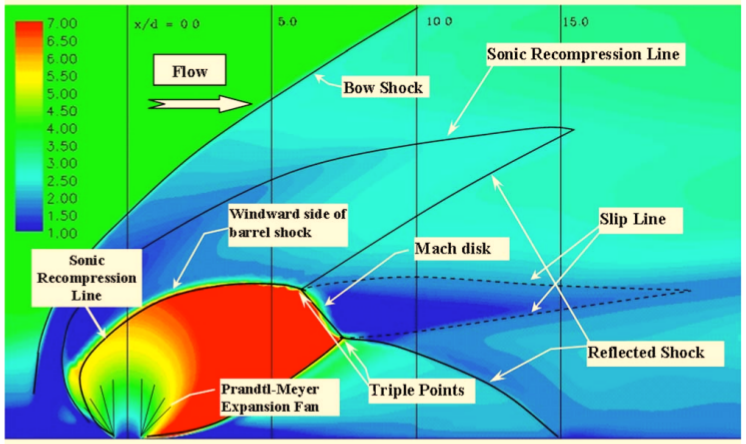
\includegraphics[width=12cm]{./chap8-3Dinjector/figs/viti-mach-scaled.png}}%
	\qquad	
	\subfigure[][Eilmer3 Simulation.]{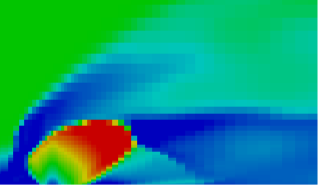
\includegraphics[width=12cm]{./chap8-3Dinjector/figs/inject-mach-profile2.png}}%
	\qquad	
	\subfigure[][Experimental (Schlieren) Results (see Viti et. al.~\protect\cite{viti2004}).]{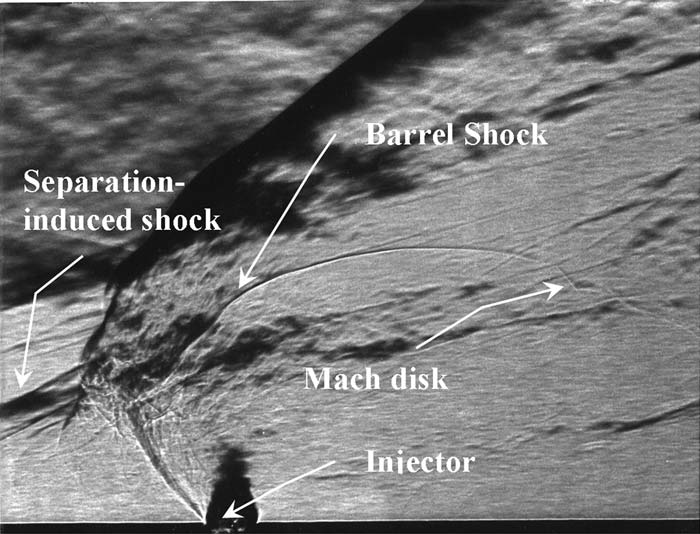
\includegraphics[width=9cm]{./chap8-3Dinjector/figs/viti-schlieren.png}}
	\caption{3D Injector Mach Number Comparison with Schlieren Imagery.}%
	\label{f:tc3:schetzcompare2}%
\end{figure}

\newpage
A graph of pressure coefficient extracted along the centreline of the flat plate surface for the latest four data entries (Figure~\ref{f:tc3:cpcentrelineovertime}) identifies that the simulation is close to reaching a steady-state solution. The $C_P$ data upstream of the injector is undergoing small changes, the most obvious of which can be identified as increasing $C_P$ entries during the second and third upstream peaks. Immediately downstream of the injector, the $C_P$ seems stable, however is still stabilising in the turbulent wake region - particularly after the reflected shock impingement on the flat plate surface ($x/D\approx14$).

A comparison of pressure coefficient along the centre of the geometry with Viti's~\cite{schetz2009} results indicate good prediction of the troughs and peaks along the full length (Figure~\ref{f:tc3:cpcentrelinefullres}). Given that the simulation is currently at $0.758$\,ms, an extended test time would allow the shocks and associated high pressure regions to shift further downstream, resulting in better correlation between the Eilmer3 and Viti solutions. 

The experimental results by Wallis~\cite{wallis2001} (obtained using pressure sensitive paint) are more accurately predicted by the Eilmer3 simulation than by Viti, as indicated by the general shape of the $C_P$ curve, and the first $C_P$ peak in Figure~\ref{f:tc3:cpcentreline}. As with the comparison to Viti's solutions, an extended test time and higher grid resolution would alter this correlation, potentially resulting in higher $C_P$ peaks occurring close to the injector.

The effects of the selection of a coarse mesh are obvious from the $C_P$ graphs, in regions where large pressure gradients are experienced, such as immediately upstream of the injector.

%
\begin{figure}[htbp]
 \begin{center}
  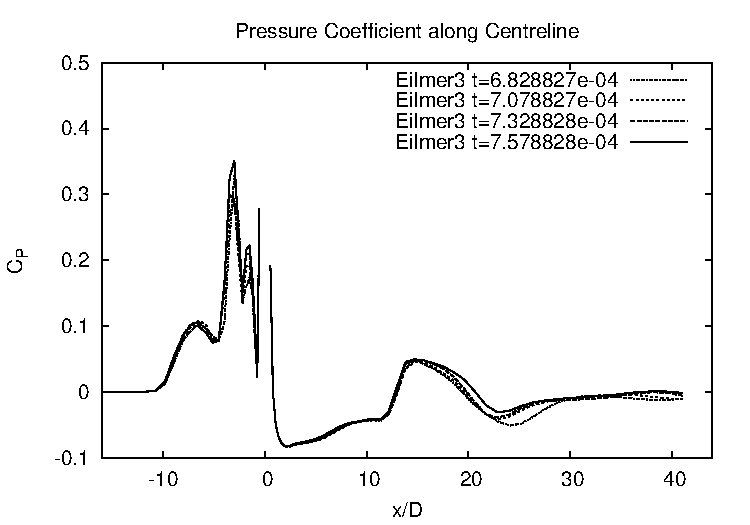
\includegraphics[width=14cm]{./chap8-3Dinjector/figs/normalisedCP_all.pdf}
  \caption{3D Injector Pressure Coefficient along Full-length Centreline (X Axis) over time.}
  \label{f:tc3:cpcentrelineovertime}
 \end{center}
\end{figure}
%
\begin{figure}[htbp]
 \begin{center}
  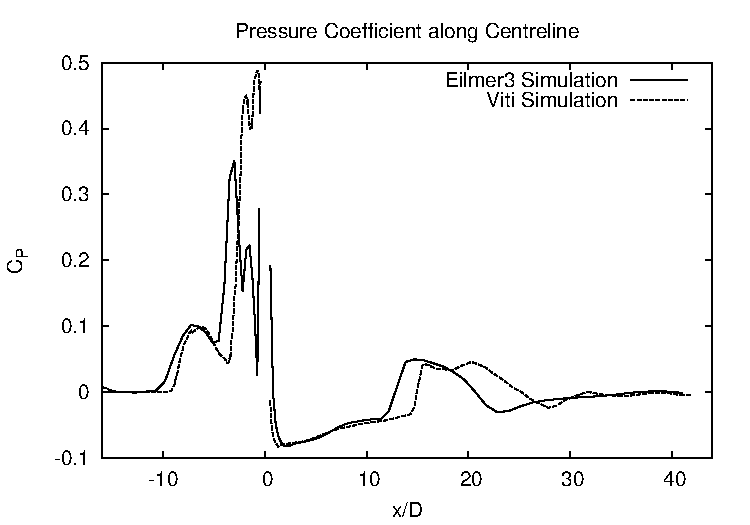
\includegraphics[width=14cm]{./chap8-3Dinjector/figs/normalisedCP_fullres.pdf}
  \caption{3D Injector Pressure Coefficient along Full-length Centreline (X Axis).}
  \label{f:tc3:cpcentrelinefullres}
 \end{center}
\end{figure}
%
%
\begin{figure}[htbp]
 \begin{center}
  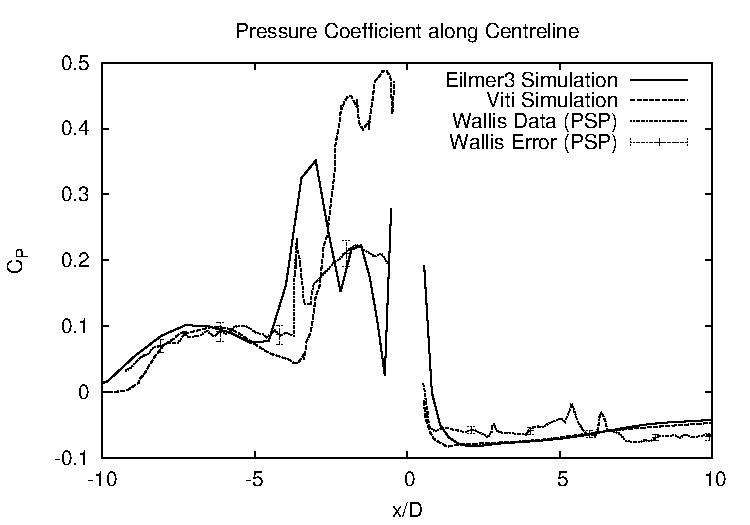
\includegraphics[width=14cm]{./chap8-3Dinjector/figs/normalisedCP.pdf}
  \caption{3D Injector Pressure Coefficient along Centreline (X Axis).}
  \label{f:tc3:cpcentreline}
 \end{center}
\end{figure}
%

\newpage
Figures~\ref{f:tc3:Cpcontours1} and~\ref{f:tc3:Cpcontours2} indicate pressure coefficient data over the surface of the flat plate, compared to Viti's simulation and Wallis' PSP solutions respectively. Both feature $C_P$ mapped over a range of $-0.1$ to $0.5$, and are contoured in increments of $0.05$ (thirteen contours total).

The correlation of both $C_P$ maps with their respective solution is excellent, however as with the centreline $C_P$ graphs, an extended simulation and steady-state solution would result in shifting of shocks further downstream, condensing the high pressure regions upstream and resulting in a more accurate prediction. 

Given that the thirteen contours are staggered in $0.05$ intervals, the $C_P$ contours in Figure~\ref{f:tc3:Cpcontours1}a are likely to match those produced by Viti (Figure~\ref{f:tc3:Cpcontours1}b) given a longer test time, allowing the contours to shift outwards from the symmetry plane. 

\begin{figure} [htbp]
	\centering
	\subfigure[][Eilmer3 Simulation.]{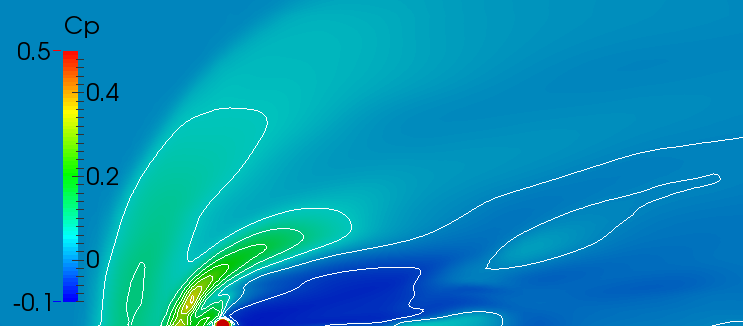
\includegraphics[width=13cm]{./chap8-3Dinjector/figs/inject-Cp-contours.png}}%
	\qquad	
	\subfigure[][Viti Simulation (see Viti et. al.~\protect\cite{schetz2009}).]{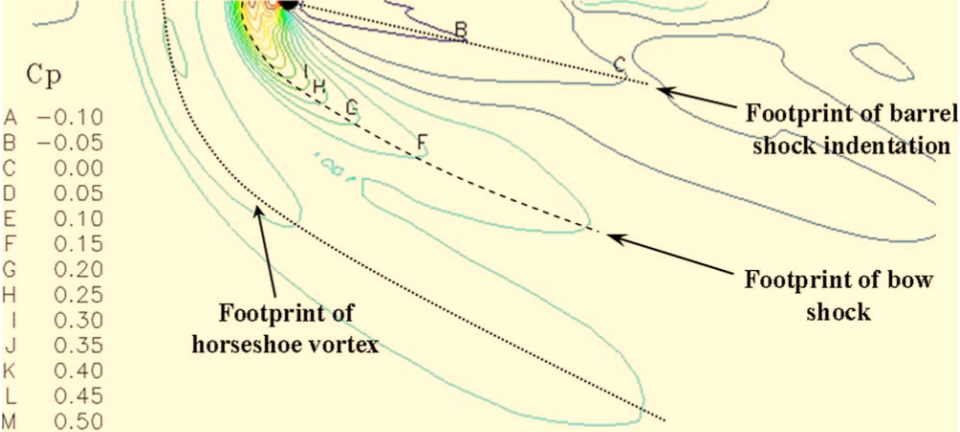
\includegraphics[width=13cm]{./chap8-3Dinjector/figs/viti-Cp-contours.png}}%
	\caption{3D Injector Pressure Coefficient over surface of flat plate.}%
	\label{f:tc3:Cpcontours1}%
\end{figure}

\begin{figure} [h]
	\centering
	\subfigure[][Experimental (PSP) Results (see Wallis~\protect\cite{wallis2001}).]{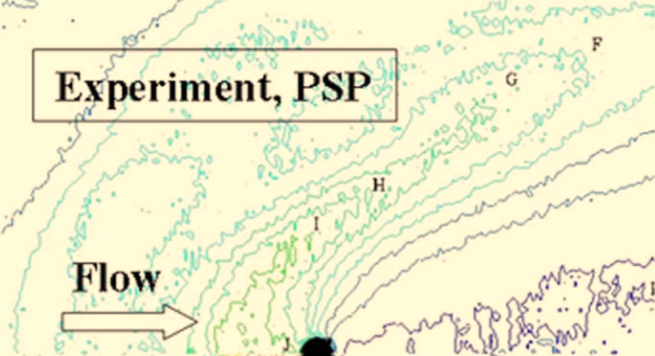
\includegraphics[width=13cm]{./chap8-3Dinjector/figs/wallis-Cp-PSP.png}}%
	\qquad	
	\subfigure[][Eilmer3 Simulation.]{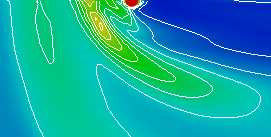
\includegraphics[width=13cm]{./chap8-3Dinjector/figs/inject-Cp-contours2.png}}%
	\caption{3D Injector Pressure Coefficient over surface of flat plate with PSP results.}%
	\label{f:tc3:Cpcontours2}%
\end{figure}

One of the major trade-offs experienced when developing three-dimensional CFD meshes is the selection of a cell-count - select a lower resolution and risk simulation instability, or select a higher resolution and experience long simulation times. In order to ensure the test case did not checker-board on the flat plate surface, the cell-count in the Y direction was increased from its previous iterations. This allowed the $k$-$\omega$ model to properly determine the turbulence properties, and thus, the fluxes and flow properties. The increase in resolution significantly increased compute-times, and to further raise the cell-count in the X and Z directions would only lengthen the simulation even further. It was for this reason that a grid convergence study for the 3D injector mesh was unable to be undertaken. 

An avenue of future work for this test case would be to continue the simulation from the latest solution, in order to achieve a steady or quasi-steady solution. Due to time restrictions and the selected mesh resolution, a fully steady solution was unable to be produced, however the progress made so far has been promising. Given more time, the simulation should produce better final results.

Alternatively, the mesh resolution could be further increased in the X and Z directions, to reduce the aliasing effects and produce a finer solution on the symmetry plane. This would allow for a precise, qualitative comparison of the shock structure on the symmetry plane, as well as a more accurate comparison of pressure coefficient along the symmetry plane centreline.